\subsection{UML diagramy}

V tejto časti sú znázornené UML diagramy navrhovanej aplikácie, ktoré vizualizujú jej štruktúru a správanie.

\begin{figure}[H]
    \centering
    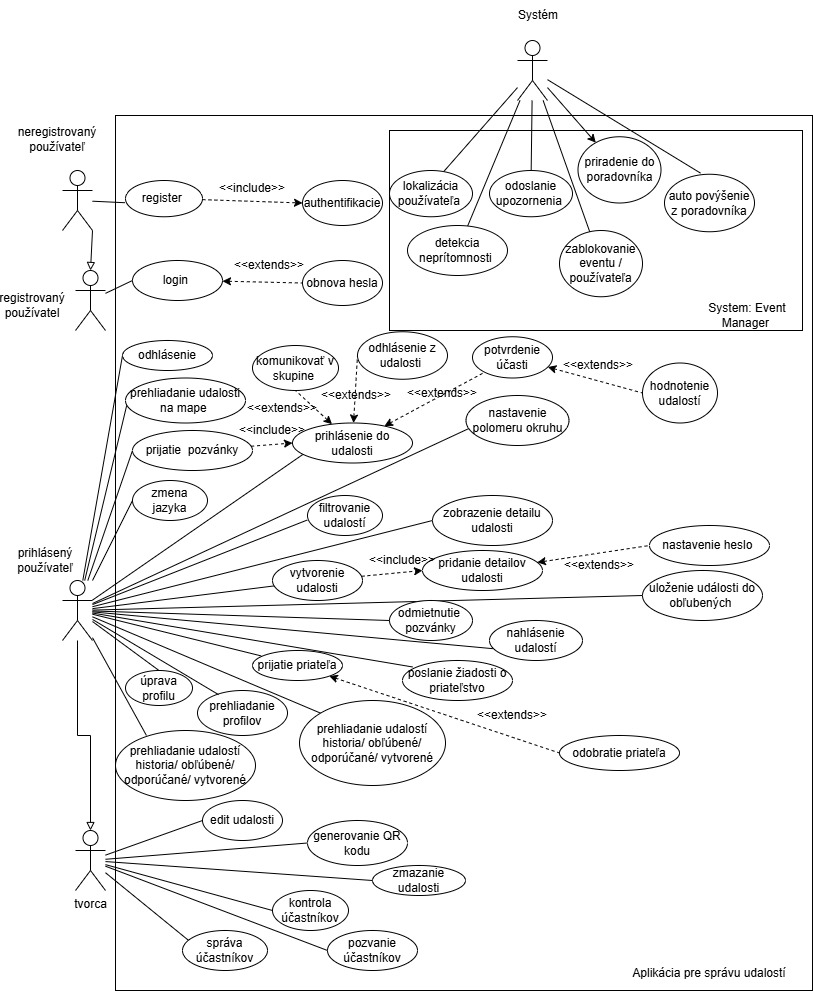
\includegraphics[width=\textwidth]{includes/navrh_riesenie/UML/use_case}
    \caption{Diagram prípadov použitia (Use Case diagram)}
    \label{fig:use_case}
\end{figure}

\begin{figure}[H]
    \centering
    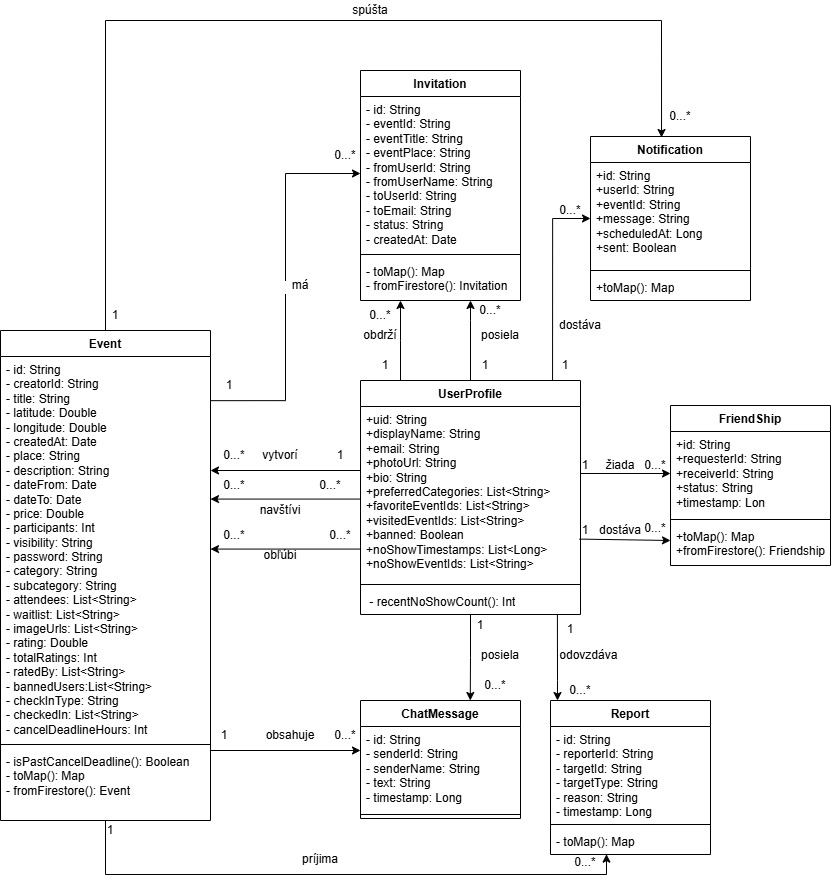
\includegraphics[width=\textwidth]{includes/navrh_riesenie/UML/class_diagram}
    \caption{Diagram tried (Class diagram)}
    \label{fig:class_diagram}
\end{figure}

\begin{figure}[H]
    \centering
    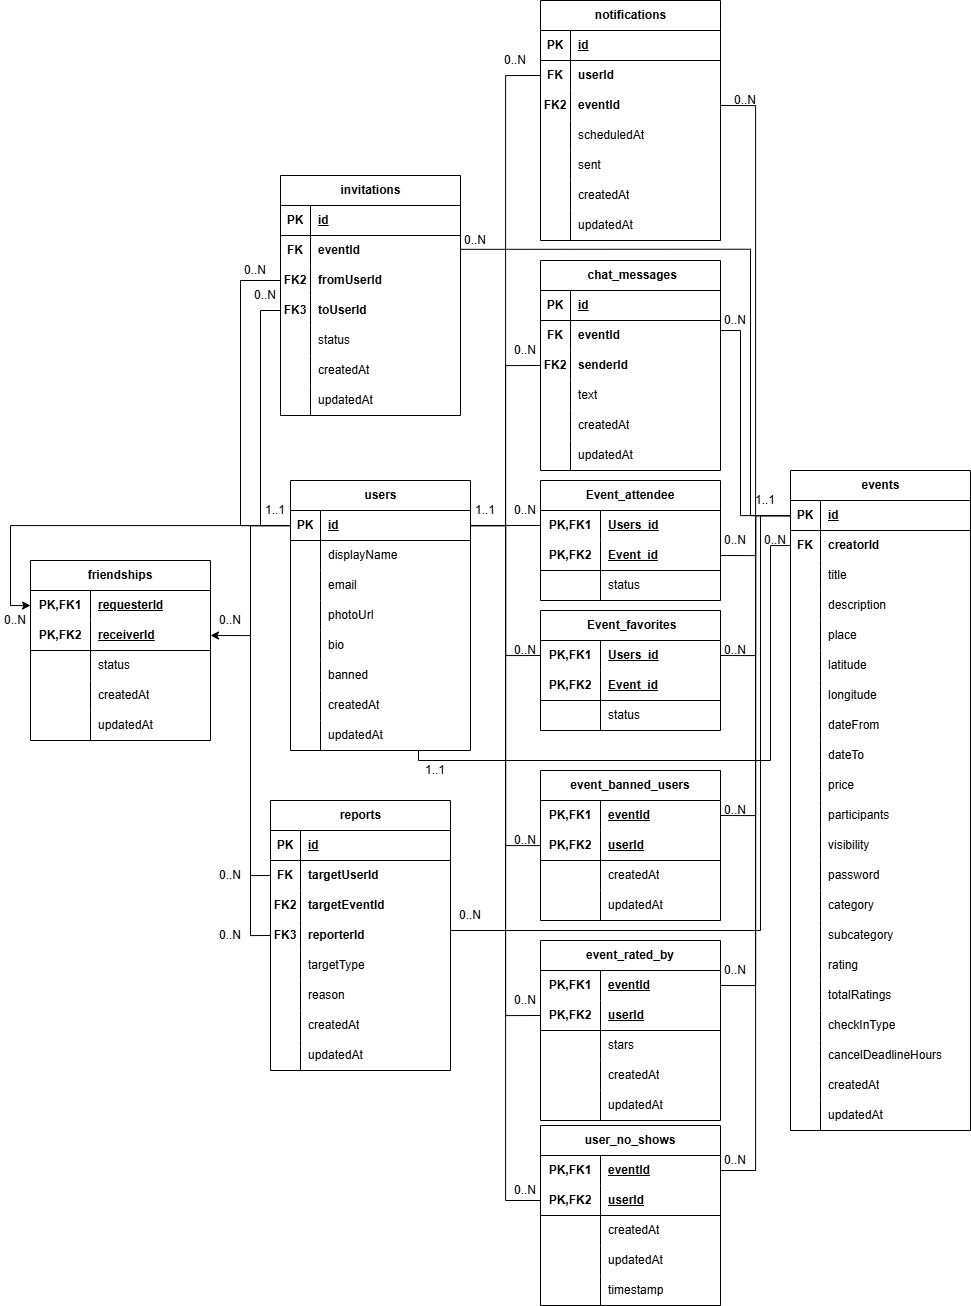
\includegraphics[width=\textwidth]{includes/navrh_riesenie/UML/relacna_databaza}
    \caption{Relačná databáza}
    \label{fig:relacna_databaza}
\end{figure}

\begin{figure}[H]
    \centering
    % Prvý obrázok
    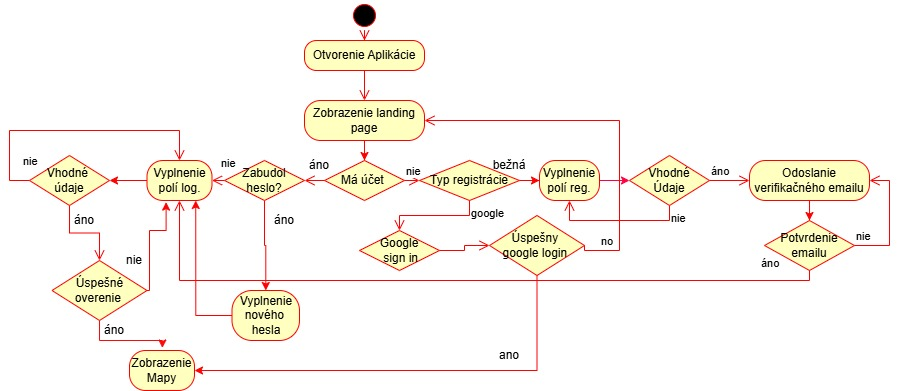
\includegraphics[width=0.75\textwidth]{includes/navrh_riesenie/UML/ActivityDiagram_auth}
    \caption{Diagram aktivít – autentifikácia}
    \label{fig:activity_auth}
    
    \vspace{1em} % Malá medzera medzi obrázkami

    % Druhý obrázok
    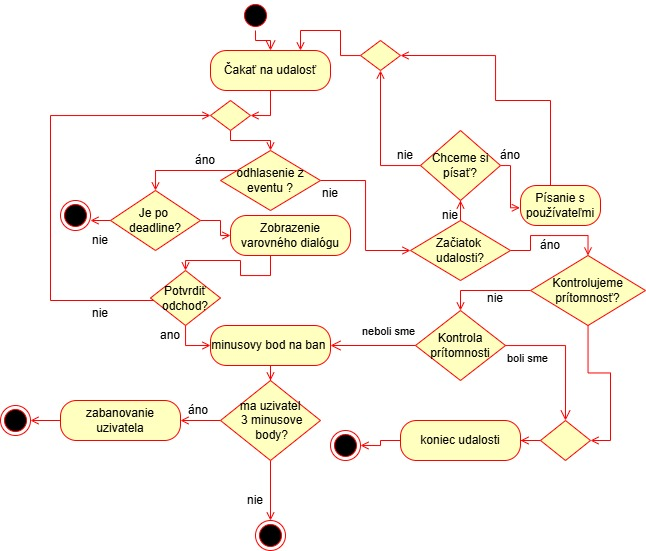
\includegraphics[width=0.75\textwidth]{includes/navrh_riesenie/UML/actiity_ucast_event}
    \caption{Diagram aktivít – účasť na udalosti}
    \label{fig:activity_ucast}
\end{figure}


\begin{figure}[H]
    \centering
    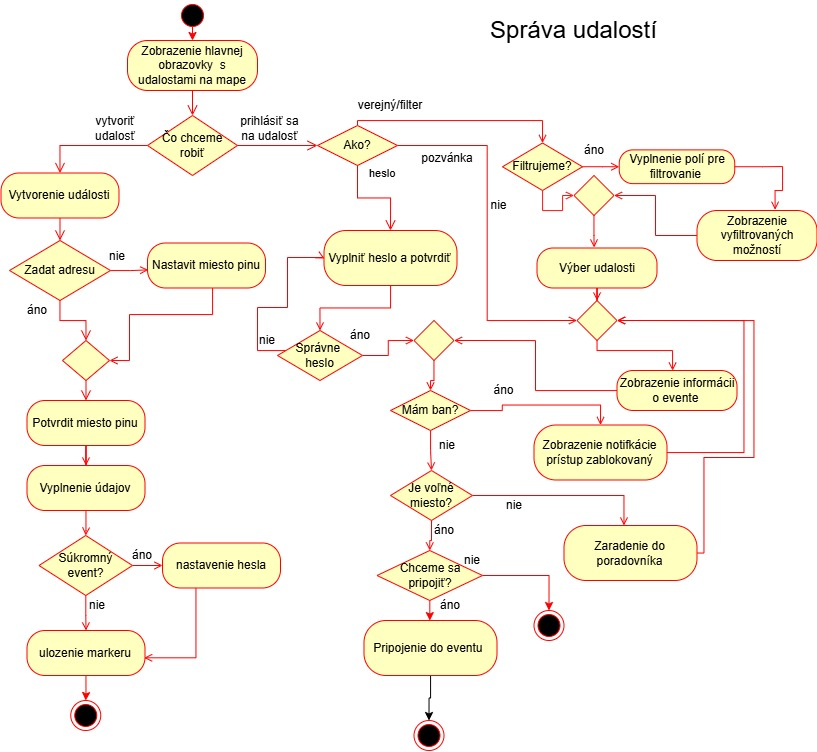
\includegraphics[width=\textwidth]{includes/navrh_riesenie/UML/activity_events}
    \caption{Diagram aktivít – správa udalostí}
    \label{fig:activity_events}
\end{figure}



\begin{figure}[H]
    \centering
    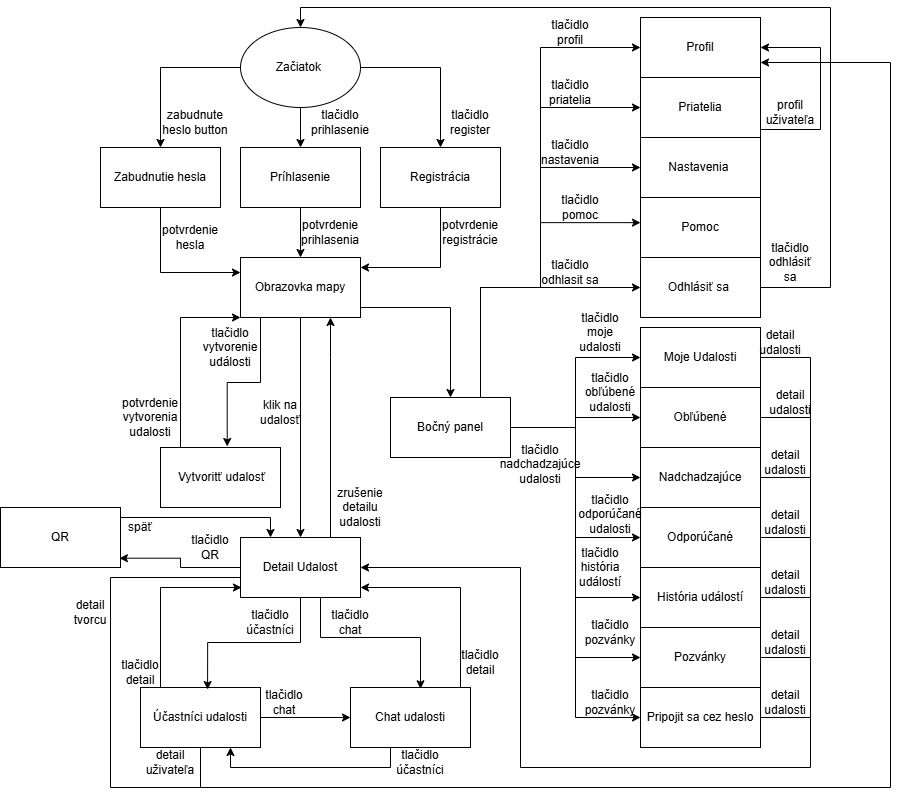
\includegraphics[width=\textwidth]{includes/navrh_riesenie/UML/NavigationBar}
    \caption{Navigačná lišta aplikácie}
    \label{fig:navigation_bar}
\end{figure}
